\documentclass[xcolor=dvipsnames,hyperref={pdfpagelabels=false}]{beamer}

\usetheme{Boadilla}

\newcommand{\bi}{\begin{itemize}}
\newcommand{\ei}{\end{itemize}}
\newcommand{\be}{\begin{enumerate}}
\newcommand{\ee}{\end{enumerate}}
\newcommand{\bc}{\begin{center}}
\newcommand{\ec}{\end{center}}
\newcommand{\bd}{\begin{description}}
\newcommand{\ed}{\end{description}}
\newcommand{\I}{\item}
\newcommand{\f}{\frame}
\newcommand{\ft}{\frametitle}

\title{A Version Management System for GlueX}
\author[Mark Ito]{Mark M.\ Ito}
\date{December 10, 2014}
\institute[JLab]{Jefferson Lab}

\begin{document}

\f{\titlepage}

\f{\ft{Use Cases}
\be
\I Communicate a consistent set of versions.
  \bi
  \I Identify working combinations
  \I Coordinate collaborative work
  \ei
\I Specify a set of versions to be built.
  \bi
  \I Green-field builds
  \I Adding versions to existing build trees
  \ei
\I Set-up environment to use specific versions.
  \bi
  \I Ensure consistency with desired set of versions.
  \ei
\ee
}

\begin{frame}[fragile]
\frametitle{XML configuration file}
\small
\begin{verbatim}
<gversions>
<package name="jana" version="0.7.2"/>
<package name="sim-recon" version="2014-09-23"/>
<package name="hdds" version="3.0"/>
<package name="cernlib" version="2005"/>
<package name="xerces-c" version="3.1.1"/>
<package name="clhep" version="2.0.4.5"/>
<package name="geant4" version="9.4"/>
<package name="root" version="5.34.04"/>
<package name="ccdb" version="1.03"/>
<package name="evio" version="4.3.1"/>
</gversions>
\end{verbatim}
\end{frame}

\f{
\ft{Standard Directory Structure}
\begin{columns}[c]
\begin{column}{2.2in}
\bi
\I Multiple versions live under generic package name
\I {\tt build\_scripts} supports this structure
\ei
\end{column}
\begin{column}{2.3in}
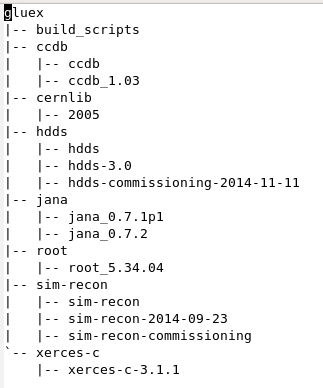
\includegraphics[width=2.3in]{directory_tree.png}
\end{column}
\end{columns}
}

\f{
\ft{generate environment variables}
\bi
\I For each package generate two environment variables
  \be
  \I version number
  \I home directory
  \ee
\I C shell and Bourne shell supported
\I build\_scripts makefiles key off version
\I gluex\_install assumes same directory structure
\I gluex\_env (in build scripts) keys off home directories
\ei
}

\begin{frame}[fragile]
\ft{example environment settings}
\footnotesize
\begin{verbatim}
setenv GLUEX_TOP /usr/local/gluex;
setenv JANA_VERSION 0.7.2;
setenv JANA_HOME /usr/local/gluex/jana/jana_0.7.2/Linux_RHEL6-x86_64-gcc4.4.7;
setenv SIM_RECON_VERSION 2014-09-23;
setenv HALLD_HOME /usr/local/gluex/sim-recon/sim-recon-2014-09-23;
setenv HDDS_VERSION 3.0;
setenv HDDS_HOME /usr/local/gluex/hdds/hdds-3.0;
\end{verbatim}
\end{frame}

\begin{frame}[fragile]
\ft{Set-Up Environment}
Example:
{\footnotesize
\begin{verbatim}
setenv GLUEX_TOP /home/username/gluex         # define top of hierarchy
setenv BUILD_SCRIPTS $GLUEX_TOP/build_scripts # define location of scripts
eval `$BUILD_SCRIPTS/version.pl version.xml`  # define versions and homes
source $BUILD_SCRIPTS/gluex_env.csh           # finish the definitions
\end{verbatim}
}
\bi
\I Environment set up for use of an existing tree. (use case \#3)
\I If tree does not exist build it with this environment (use case \#2)
\ei
{\footnotesize
\begin{verbatim}
cd $GLUEX_TOP                                 # go to the top directory
make -f $BUILD_SCRIPTS/Makefile_all gluex     # build all gluex-specific
                                              # packages
\end{verbatim}
}
\end{frame}

\begin{frame}[fragile]
\ft{Customization for Non-Standard Directories}
\bi
\I What if some package(s) not in the standard place?
\I Home area definitions can be over-ridden explicitly.
\I Subsequent invocation of {\tt gluex\_env.(c)sh} will respect incoming definitions.
\ei
{\footnotesize
\begin{verbatim}
setenv GLUEX_TOP /home/username/gluex         # define top of hierarchy
setenv BUILD_SCRIPTS $GLUEX_TOP/build_scripts # define location of scripts
eval `$BUILD_SCRIPTS/version.pl version.xml`  # define versions and homes
setenv ROOTSYS /opt/root/custom_version       # use a custom version of
                                              # ROOT
source $BUILD_SCRIPTS/gluex_env.csh           # finish the definitions
\end{verbatim}
Note: possible implications for consistency checking...
}
\end{frame}

\begin{frame}[fragile]
\ft{Adding to Existing Directory Tree}
\bi
\I Assume {\tt version\_my.xml} has alternate combination of versions.
\I Assume that {\tt /home/username/gluex} hierarchy already built once.
\ei
{\footnotesize
\begin{verbatim}
setenv GLUEX_TOP /home/username/gluex           # define top of hierarchy
setenv BUILD_SCRIPTS $GLUEX_TOP/build_scripts   # define location of
                                                # scripts
eval `$BUILD_SCRIPTS/version.pl version_my.xml` # define custom versions
source $BUILD_SCRIPTS/gluex_env.csh             # finish the definitions
cd $GLUEX_TOP                                   # go to the top directory
make -f $BUILD_SCRIPTS/Makefile_all gluex       # build all gluex-specific
                                                # packages
\end{verbatim}
}
\end{frame}

\begin{frame}[fragile]
\ft{Consistency Checking}
\bi
\I {\tt build\_scripts} creates a partial xml file in each built directory, e. g. {\tt sim-recon\_prereqs\_version.xml}:
\ei
{\footnotesize
\begin{verbatim}
<gversion version="1.0"
><package name="evio" version="4.3.1"
 /><package name="cernlib" version="2005"
 /><package name="xerces-c" version="3.1.1"
 /><package name="root" version="5.34.04"
 /><package name="jana" version="0.7.2"
 /><package name="hdds" version="3.0"
 /><package name="ccdb" version="1.03"
 /></gversion
>
\end{verbatim}
}
\bi
\I For each package with prereq xml file, version identified in xml file is checked against name of home directory from environment.
\I Inconsistencies generate warnings (at present).
\ei
\end{frame}

\f{
\ft{Conclusions}

Summary
\bi
\I System supports all three use cases:
  \be
  \I Communication
  \I Building
  \I Use
  \ee
\I Already incorporated into {\tt gluex\_install}.
\I Features have been alpha tested.
\ei
Future Work
\bi
\I follow ``prod'' links when checking consistency
\I version xml file management system
  \bi
  \I version numbers?
  \I subversion control?
  \I distribution system?
  \ei
\I decide on action to take on discovery of inconsistency
\I scheme for concurrent versions of fixed package version built with different prerequisites
\I documentation
\ei
}

\end{document}
